\documentclass[conference]{IEEEtran}
\IEEEoverridecommandlockouts
\usepackage{cite}
\usepackage{amsmath,amssymb,amsfonts}
\usepackage{graphicx}
\usepackage{array}
\usepackage{textcomp}
\usepackage{xcolor}
\usepackage[hidelinks]{hyperref}
\begin{document}

\title{TruthLens: An Evidence-Oriented Multimodal Platform for Detecting AI-Generated Media}

\author{
\IEEEauthorblockN{Manini Jaiswal, Rudrapratap Shinde, Atharva Pethkar, Soham Thakur}
\IEEEauthorblockA{\textit{Dept. of Information Technology} \\ \textit{Vidyalankar Institute of Technology} \\ Mumbai, India}
}

\maketitle

\begin{abstract}
Free image generators, face-swap apps and voice-cloning services have made synthetic media cheap to produce and hard to spot by eye. We present TruthLens, a web platform that examines an uploaded image, video or audio file and returns a banded verdict (REAL, UNCERTAIN or FAKE) together with the evidence behind it. Images are scored by a ConvNeXt-Tiny classifier and a CLIP ViT-B/16 probe whose fake probabilities are combined with a maximum rule; videos by an EfficientNet-B0 applied to 16 face crops; speech by a fine-tuned wav2vec 2.0 model over 4-s windows. Every verdict is shipped with Grad-CAM maps or per-frame and per-window scores, C2PA Content Credential validation, metadata and Stable Diffusion watermark checks, a temperature-scaled confidence and a PDF report. We evaluate the deployed models separately on sources seen and unseen in training. On 4,000 images from training-distribution sources the image ensemble reaches 98.4\% accuracy (AUC 1.00); on 2,517 images from unseen generators it falls to 53.2\% (AUC 0.67). The video model attains AUC 0.892 on 300 unseen face-swap clips, yet drops to chance or below under heavy JPEG compression, blur and down-scaling. Embedded Content Credentials identified all eight ChatGPT images that every classifier called REAL, but none survived a re-encode. We argue that detector scores should be presented as one strand of evidence, not as a final answer.
\end{abstract}

\begin{IEEEkeywords}
Deepfake detection, AI-generated images, multimodal media forensics, explainable AI, content provenance, C2PA, calibration, robustness
\end{IEEEkeywords}


\section{Introduction}
\IEEEPARstart{M}{AKING} a convincing fake photograph used to take hours with editing software. It now takes a one-line prompt. Diffusion models render photorealistic scenes, consumer face-swap apps replace a face in a phone video within minutes, and voice-cloning services need only a short sample of the target speaker. Journalists, fact-checkers, teachers and ordinary users are increasingly asked to decide whether a file is genuine, usually without any forensic training.

Detection research is active but split by modality, each with its own benchmarks: FaceForensics++~\cite{ffpp} and Celeb-DF~\cite{celebdf} for face video, CIFAKE~\cite{cifake} and GenImage~\cite{genimage} for images, and ASVspoof~\cite{asvspoof2019} for speech. Two problems appear as soon as such models are put in front of users. First, detectors trained on one family of generators transfer poorly to others~\cite{wang2020,ojha2023,genimage}, so benchmark accuracy overstates what a user will experience. Second, a bare probability gives the user nothing to check: a score of 0.97 says neither why the model is suspicious nor whether the file itself carries information about its origin.

TruthLens is our response to both problems. It is a working web application that routes each upload to a modality-specific detector, then surrounds the score with evidence the user can inspect. This paper describes the implemented system and, just as importantly, measures where it fails. Our contributions are:

\begin{itemize}
\item a deployed platform covering images, video and speech, with detectors trained or fine-tuned by the authors and a common verdict, report and history layer;
\item an evidence layer that combines Grad-CAM and saliency explanations, C2PA provenance, metadata and watermark checks, and calibrated confidence, while never letting missing provenance count as proof of authenticity;
\item an evaluation of the deployed models that keeps seen and unseen data sources apart and adds tests of robustness to 20 degradations, explanation faithfulness, provenance survival and per-group error rates; and
\item a candid account of negative results, including two generator blind spots, three unsuccessful video preprocessing variants and a collapse of the video model under compression.
\end{itemize}

Section II reviews related work. Section III describes the detectors and the evidence layer, and Section IV the implementation. Sections V and VI give the evaluation protocol and results. Section VII discusses limitations, and Section VIII concludes.


\section{Related Work}
\subsection{AI-Generated Image Detection}
Wang et al.~\cite{wang2020} showed that a ResNet trained on images from a single GAN, with blur and JPEG augmentation, transfers surprisingly well to other GANs of that period. Frank et al.~\cite{frank2020} found that up-sampling layers leave traces in the frequency spectrum. With diffusion models the picture changed: GenImage~\cite{genimage} reports large accuracy drops when detectors are tested on generators they were not trained on. Ojha et al.~\cite{ojha2023} proposed classifying frozen CLIP~\cite{clip} features with a light head, which generalises better than end-to-end training because the feature space is not shaped around one generator. Our image branch combines both ideas: a ConvNeXt~\cite{convnext} classifier trained end to end and a CLIP probe.

\subsection{Face-Manipulation Video Detection}
FaceForensics++~\cite{ffpp} introduced a benchmark of four manipulation methods with an XceptionNet baseline. Celeb-DF~\cite{celebdf}, the DFDC dataset~\cite{dfdc} and WildDeepfake~\cite{wilddeepfake} added harder, more varied and in-the-wild forgeries. Most practical detectors crop the face and classify frames with an ImageNet-pretrained CNN, with EfficientNet~\cite{efficientnet} variants common among strong DFDC entries~\cite{dfdc}. The weak point of this design is the face detector: if it finds the wrong region, the classifier never sees the manipulation, a failure we observe directly in Section VI.

\subsection{Synthetic Speech Detection}
ASVspoof 2019~\cite{asvspoof2019} established logical-access spoofing benchmarks, and graph-attention models such as AASIST~\cite{aasist} perform strongly on them. M\"uller et al.~\cite{inthewild} showed that such models degrade sharply on real-world recordings. Self-supervised front-ends such as wav2vec 2.0~\cite{wav2vec2} improve generalisation when fine-tuned for spoofing detection~\cite{tak2022}, which motivates our choice of audio backbone.

\subsection{Explanation, Provenance and Calibration}
Grad-CAM~\cite{gradcam} and gradient saliency~\cite{simonyan2014} highlight the inputs a network's output depends on, but do not by themselves prove manipulation. Provenance answers a different question: the C2PA specification~\cite{c2pa} lets a camera or generator cryptographically sign a manifest that records how a file was made. Stable Diffusion's reference code also embeds a fixed invisible watermark~\cite{ldm,invisiblewm}, and error level analysis (ELA)~\cite{krawetz2007} visualises JPEG recompression differences. Modern networks are often over-confident, and temperature scaling~\cite{guo2017} is a simple post-hoc fix. Individually these tools are well known; what is rarely reported is how they behave together in a deployed system and how each fails.


\section{System Design}
\subsection{Overview}
Fig. \ref{fig-arch} shows the request path. The client uploads a file of up to 100 MB. The gateway checks the declared MIME type against the file's leading bytes, stores the file and creates a database record. Detection is then dispatched by media type. Image and audio scans complete within the request; video scans run as background jobs that report real progress from frame decoding, face cropping and scoring. Explanations and provenance are computed on demand by separate endpoints, so a failure in either never affects the stored verdict.

\begin{figure}[!t]
\centering
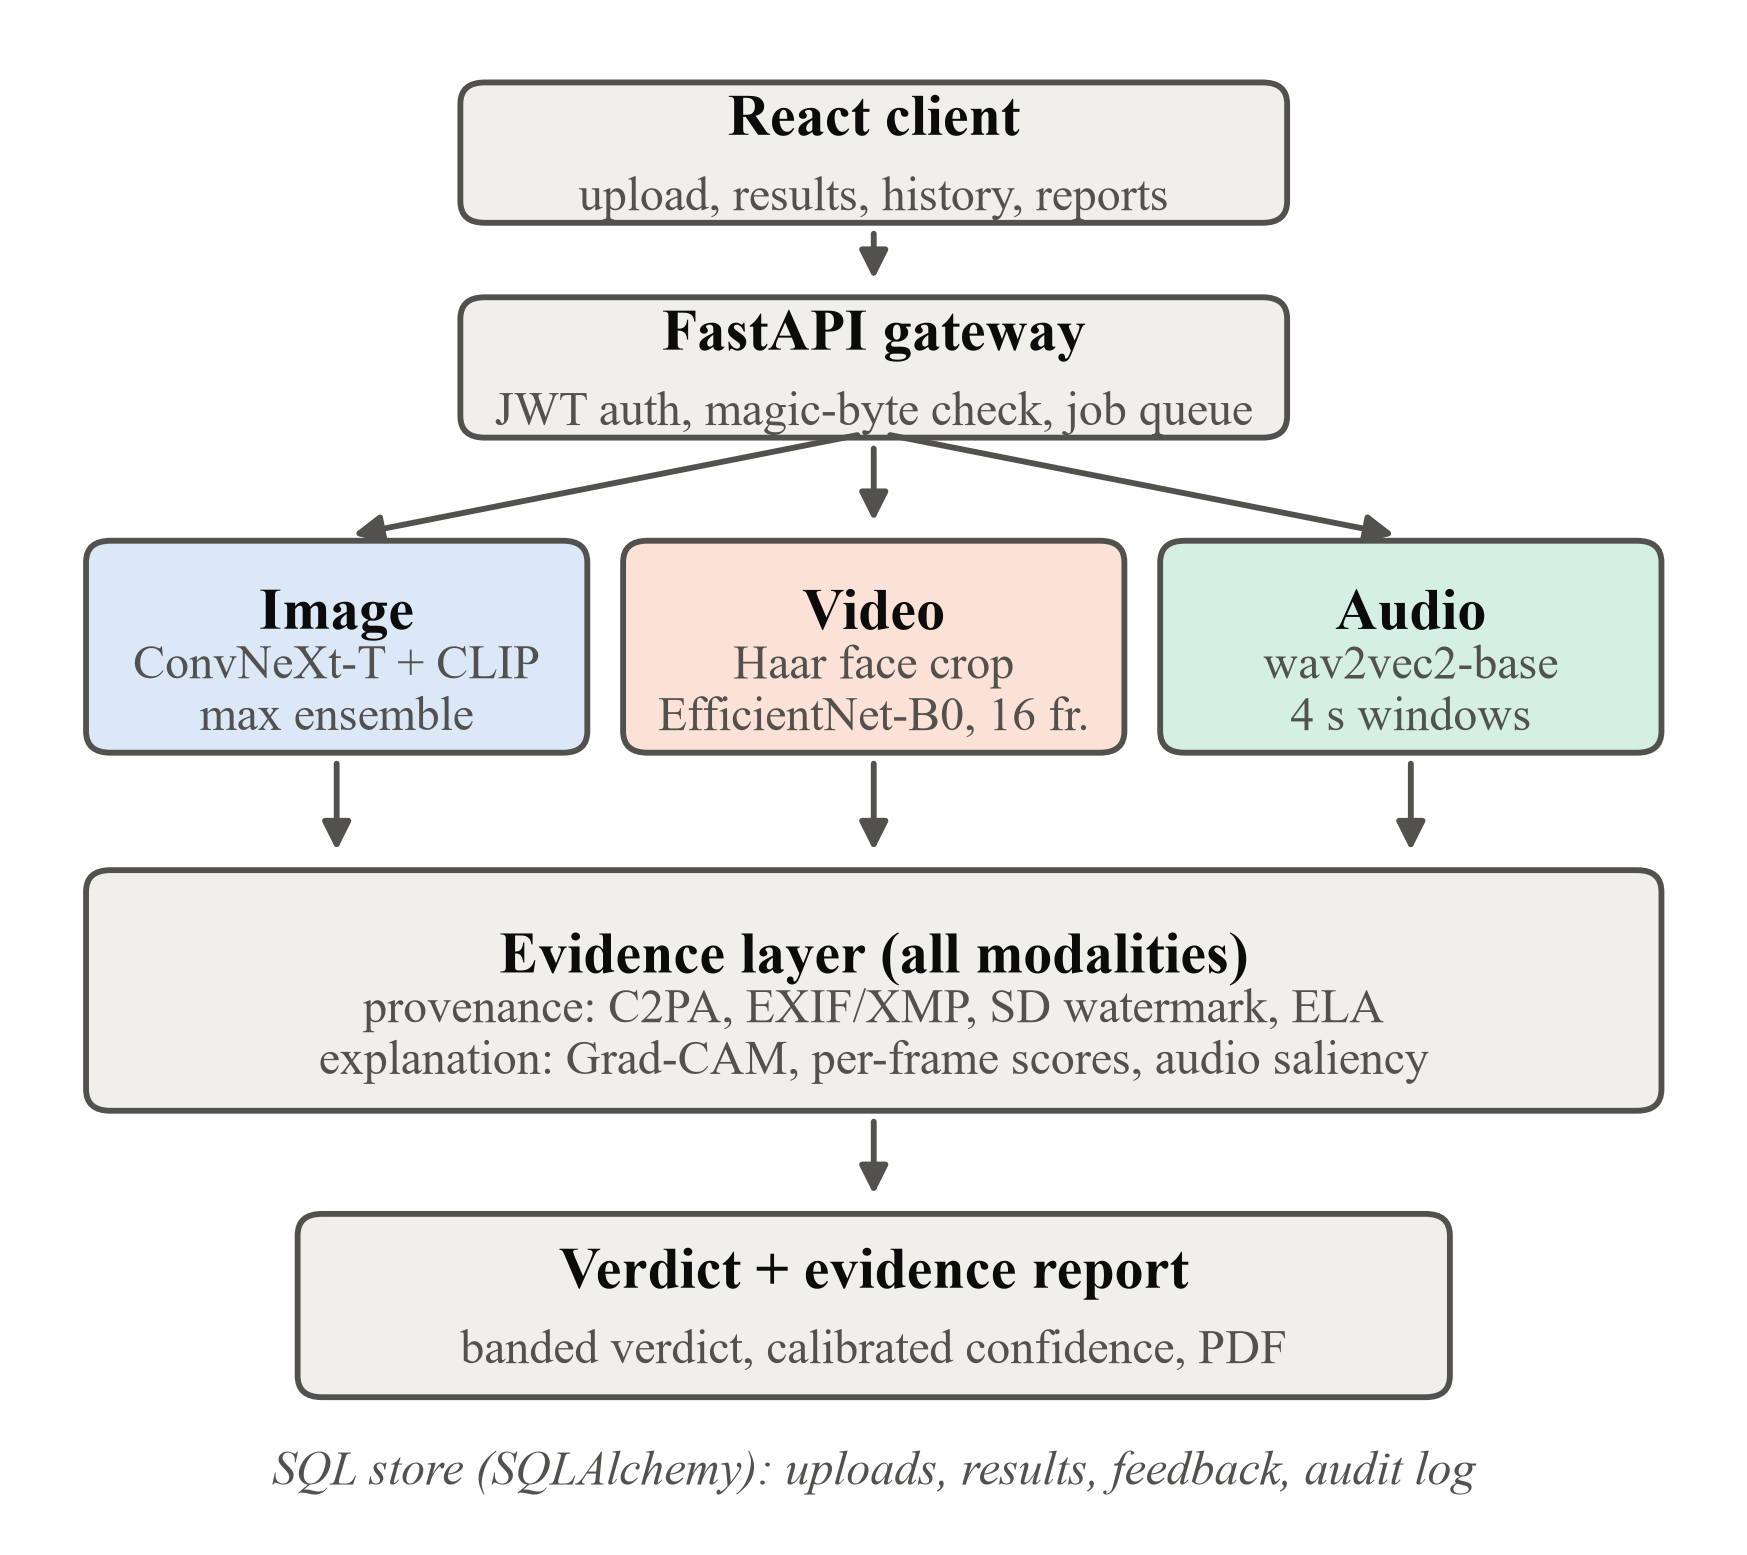
\includegraphics[width=\columnwidth]{figures/fig1_architecture.png}
\caption{TruthLens architecture. Each upload is routed to one modality detector; all three share the evidence layer and the verdict and report stage.}
\label{fig-arch}
\end{figure}

\subsection{Image Detector}
The first sub-model is ConvNeXt-Tiny~\cite{convnext}. It was first trained on CIFAKE~\cite{cifake}, then fine-tuned on four sources: CIFAKE, the AI-vs-Human-Generated dataset~\cite{aivshuman}, 140k Real and Fake Faces~\cite{faces140k} and DeepDetect-2025~\cite{deepdetect} (StyleGAN3, DALL-E 3, Midjourney and SD3 images). Training used random JPEG re-compression, blur and resize augmentation. Inputs are resized directly to 224$\times$224. An earlier variant first reduced images to 32$\times$32 to match CIFAKE; on a held-out evaluation of 3,000 images per source this cut face-image accuracy from 99.8\% to 57\%, so it was removed.

The second sub-model is a frozen CLIP ViT-B/16~\cite{clip} backbone with a small trained MLP head, following~\cite{ojha2023}. Its head was trained on the same four sources plus 257 hand-reviewed Stable Diffusion images retrieved from DiffusionDB~\cite{diffusiondb} by prompt text (vintage-photo and period-costume portraits). We added that set after finding that both sub-models labelled stylised ``portrait-app'' images REAL with over 99.9\% confidence.

With p\_C and p\_L denoting the FAKE probabilities of ConvNeXt and CLIP, the ensemble score is

\begin{equation}
p_{\mathrm{img}} = \max\left(p_{C},\, p_{L}\right).
\end{equation}

We chose the maximum over the mean deliberately. ConvNeXt was not retrained on the portrait genre and remains blind to it (6.7\% caught); averaging diluted CLIP's 93.3\% on that genre to 66.7\%. The maximum keeps either model's detection, at the cost of more false alarms on real photographs (Section VI-A).

\subsection{Video Detector}
Sixteen frames are sampled at evenly spaced indices. In each frame a Haar cascade~\cite{violajones} locates the largest frontal face, the box is enlarged by 20\%, and the crop is resized to 224$\times$224 with bilinear interpolation and ImageNet normalisation. If no face is found, a centre square is used instead. An EfficientNet-B0~\cite{efficientnet} produces one FAKE logit per frame; the video score is the sigmoid of the mean logit, compared with a threshold of 0.525 taken from the model's original Celeb-DF v2 evaluation protocol. The system also reports how many of the 16 frames contained a detected face and warns the user when fewer than half did, because such verdicts rest on generic crops.

\subsection{Audio Detector}
Speech is decoded to 16 kHz mono and RMS-normalised over the whole clip. Up to six 4-s windows are taken at evenly spaced offsets, and shorter clips are tiled to length. A wav2vec 2.0 base model~\cite{wav2vec2} with mean-pooled hidden states and a linear head returns a deepfake probability per window; the clip score is their mean. The model was fine-tuned in successive rounds on voice-conversion attacks from ASVspoof 2019~\cite{asvspoof2019}, DEEP-VOICE~\cite{deepvoice}, In-the-Wild~\cite{inthewild} (split by speaker), genuine LibriSpeech~\cite{librispeech} narration (split by speaker, added to remove false alarms on clean studio audio) and a range of VCC 2020~\cite{vcc2020} voice-conversion systems (split by system). A pretrained AASIST~\cite{aasist} model remains available as a fallback.

\subsection{Verdict Bands and Calibrated Confidence}
All three detectors map their score $p$ to a three-way verdict around their threshold $t$ (0.5 for image and audio, 0.525 for video):

\begin{equation}
v(p) = \begin{cases} \text{FAKE}, & p \geq t + 0.2 \\ \text{REAL}, & p \leq t - 0.2 \\ \text{UNCERTAIN}, & \text{otherwise.} \end{cases}
\end{equation}

The UNCERTAIN band reflects a deliberate choice that a borderline score should be reported as borderline rather than forced into a binary answer. The raw score is shown, and next to it a temperature-scaled confidence~\cite{guo2017},

\begin{equation}
\hat{p} = \sigma\!\left(\operatorname{logit}(p)\,/\,T\right),
\end{equation}

where $T$ is fitted per modality by minimising negative log-likelihood on labelled evaluation scores ($T=$ 4.45 for images, 0.116 for video). No audio temperature has been fitted because no labelled audio evaluation set exists in the harness yet. The interface shows ``not available'' in that case rather than a guessed value.

\subsection{Explanation Layer}
For images, Grad-CAM~\cite{gradcam} is computed on ConvNeXt's last stage with respect to the FAKE logit. Because a per-image normalised Grad-CAM map always shows some bright region, even on images the model considers real, we scale the map's intensity by ConvNeXt's own FAKE probability, so a confident REAL verdict shows a near-empty map. CLIP has no spatial map; when CLIP alone drives a FAKE verdict the interface says so instead of displaying ConvNeXt's map as if it explained the result. For video the user sees each frame's probability, the exact crops the model received and Grad-CAM on the three most suspicious frames. For audio, Grad-CAM does not apply because wav2vec 2.0 has no late two-dimensional feature map, so we use input-gradient saliency~\cite{simonyan2014} pooled into 80 time bins and overlaid on the spectrogram of the most suspicious window.

\subsection{Provenance Layer}
The provenance service runs independently of the detectors and reports four kinds of evidence. (i) C2PA manifests~\cite{c2pa} are validated with the official SDK against the published trust list. The service reports whether the signature is valid, whether the file is unchanged since signing, whether the signer is trusted, and whether the manifest declares AI generation through the IPTC digital-source-type field. (ii) Embedded metadata: camera EXIF, editing software, the presence (never the coordinates) of GPS data, and generation parameters left by Stable Diffusion front-ends. (iii) The fixed 48-bit DWT-DCT watermark that Stable Diffusion's reference pipeline embeds~\cite{invisiblewm}. We re-implemented the decoder, verified it bit-for-bit against the reference library and require an exact 48/48 match. For video, eight sampled frames are checked. (iv) ELA for JPEG files, shown as a visual aid only and never scored.

Provenance never changes the verdict, because metadata can be removed by any re-save. A present AI declaration is strong evidence. An absent one says nothing either way. When the detector says REAL but the file declares itself AI-generated, the interface and report show an explicit conflict note.


\section{Implementation}
The client is written in React with Vite, with each route loaded lazily. The backend is an asynchronous FastAPI service using SQLAlchemy, which defaults to SQLite and accepts any SQLAlchemy database URL. Inference uses PyTorch, open\_clip, Hugging Face Transformers and OpenCV, and PDF reports are generated with ReportLab. Authentication uses bcrypt password hashes and HS256 JSON Web Tokens with a 24-hour expiry. Every resource is owner-scoped, and other users receive 404 rather than 403, so the existence of an upload is not revealed. The production configuration places Nginx in front of the API with a content-security policy and per-IP rate limits: 10 requests per minute on authentication and 20 per minute on upload and detection. The server refuses to start in production mode with a default signing key. Users can give ``was this correct?'' feedback, and only items for which they tick an opt-in box can be exported for evaluation. Users can also delete their account together with every file and report. Every response carries a request ID that is echoed in error messages, and security-relevant actions are written to an audit log.

Video jobs use an in-process queue with a concurrency of one, because CPU inference is the bottleneck. Progress is reported from decoding (0--70\%), face cropping (70--90\%) and scoring, and a job can be cancelled. After loading and warm-up, all image and video models together occupy about 265 MB of resident memory on CPU. The backend has 271 automated tests that run without model checkpoints, plus checkpoint-dependent tests that reproduce the production scores exactly. A mutation script checks that the tests guarding 17 critical behaviours, such as the thresholds, ownership checks and consent gating, fail when that behaviour is broken.


\section{Evaluation Protocol}
All measurements use the production detector classes with unchanged weights and thresholds. Each data source is tagged \emph{seen} if the model was trained on data from it and \emph{unseen} otherwise. Results are reported separately for each group, because pooled accuracy depends mainly on how many files of each kind were sampled. Table \ref{tab-data} lists the sources. We report accuracy, recall on fakes, specificity on real files, ROC-AUC with 95\% bootstrap intervals (1,000 resamples) and expected calibration error (ECE, 10 bins). The metric code was checked against scikit-learn and agrees to within $2\times10^{-16}$.

\begin{table}[!t]
\renewcommand{\arraystretch}{1.15}
\caption{Evaluation data. Seen = model trained on this source.}
\label{tab-data}
\centering
\footnotesize
\setlength{\tabcolsep}{3pt}
\begin{tabular}{>{\raggedright\arraybackslash}p{0.57\columnwidth}>{\raggedright\arraybackslash}p{0.20\columnwidth}>{\raggedright\arraybackslash}p{0.15\columnwidth}}
\hline
\textbf{Source} & \textbf{Files} & \textbf{Status} \\
\hline
CIFAKE~\cite{cifake}, AI-vs-Human~\cite{aivshuman}, 140k Faces~\cite{faces140k}, DeepDetect~\cite{deepdetect} & 4,000 & Seen \\
GenImage~\cite{genimage}: real / SD / Midjourney / BigGAN & 600 / 300 / 300 / 300 & Unseen \\
OpenFake~\cite{openfake}: real / fake & 500 / 500 & Unseen \\
ChatGPT ``everyday'' photos; own photos & 8; 9 & Unseen \\
Portrait-app images & 15 & CLIP only \\
RTFS-10k~\cite{rtfs}: real / inswapper / uniface & 150 / 75 / 75 & Unseen \\
Own videos (incl. Akool, Magic Hour fakes) & 10 & Unseen \\
UTKFace~\cite{utkface} real faces, 10 gender $\times$ race groups & 600 & Unseen \\
\hline
\end{tabular}
\end{table}

Robustness was measured on 300 label-balanced images (180 seen, 120 unseen) under 21 settings. These were the clean images, JPEG quality 90 to 10, down-scaling and restoring to 75--25\%, Gaussian blur (sigma 0.5--3), additive noise (std 5--20), centre crops of 80\% and 60\%, and screenshot, WhatsApp-style (longest side 1600 px, JPEG q65) and WebP pipelines, following the corruption methodology of~\cite{hendrycks2019}. For video, the same perturbation functions were applied in memory to all 16 sampled frames of 30 RTFS clips (10 per class) under 11 settings. All inference ran on CPU.


\section{Results}
\subsection{Images: Seen Versus Unseen Sources}
\begin{table}[!t]
\renewcommand{\arraystretch}{1.15}
\caption{Image detection by training status (threshold 0.5).}
\label{tab-image}
\centering
\footnotesize
\setlength{\tabcolsep}{3pt}
\begin{tabular}{>{\raggedright\arraybackslash}p{0.28\columnwidth}>{\raggedright\arraybackslash}p{0.15\columnwidth}>{\raggedright\arraybackslash}p{0.11\columnwidth}>{\raggedright\arraybackslash}p{0.13\columnwidth}>{\raggedright\arraybackslash}p{0.11\columnwidth}>{\raggedright\arraybackslash}p{0.15\columnwidth}}
\hline
\textbf{System} & \textbf{Data} & \textbf{Acc.} & \textbf{Recall} & \textbf{Spec.} & \textbf{AUC} \\
\hline
ConvNeXt & Seen & 99.3 & 99.5 & 99.2 & 1.000 \\
CLIP & Seen & 97.6 & 97.8 & 97.5 & 0.997 \\
Mean & Seen & 99.6 & 99.8 & 99.4 & 1.000 \\
Max (deployed) & Seen & 98.4 & 100.0 & 96.8 & 1.000 \\
ConvNeXt & Unseen & 50.2 & 12.0 & 98.7 & 0.665 \\
CLIP & Unseen & 49.7 & 20.6 & 86.7 & 0.640 \\
Mean & Unseen & 48.5 & 10.9 & 96.3 & 0.670 \\
Max (deployed) & Unseen & 53.2 & 27.3 & 86.0 & 0.665 \\
\hline
\end{tabular}
\end{table}

Table \ref{tab-image} contains the central result of this work. On seen sources every configuration is near perfect. On unseen generators the deployed ensemble catches only 27.3\% of fakes, and AUC drops to 0.665. Per source, it catches 30.7\% of GenImage Stable Diffusion images, 20.0\% of Midjourney and 26.0\% of BigGAN images, and reaches 54.3\% accuracy on OpenFake. All eight photorealistic ChatGPT images were labelled REAL with more than 99.99\% confidence. The maximum rule trades specificity for recall: compared with the mean, it raises unseen-fake recall from 10.9\% to 27.3\% but lowers real-photo specificity from 96.3\% to 86.0\%. On the portrait-app genre it keeps CLIP's 93.3\%. The seen-source figures should be read as measures of fit, because the exact training hold-out split was not recorded.

\subsection{Video}
\begin{table}[!t]
\renewcommand{\arraystretch}{1.15}
\caption{Video detection on 300 unseen RTFS clips: deployed pipeline and three preprocessing variants.}
\label{tab-video}
\centering
\footnotesize
\setlength{\tabcolsep}{3pt}
\begin{tabular}{>{\raggedright\arraybackslash}p{0.37\columnwidth}>{\raggedright\arraybackslash}p{0.13\columnwidth}>{\raggedright\arraybackslash}p{0.15\columnwidth}>{\raggedright\arraybackslash}p{0.13\columnwidth}>{\raggedright\arraybackslash}p{0.15\columnwidth}}
\hline
\textbf{Pipeline} & \textbf{Acc.} & \textbf{Recall} & \textbf{Spec.} & \textbf{AUC} \\
\hline
Deployed (Haar, 20\% pad) & 79.3 & 74.7 & 84.0 & 0.895 \\
+ rotation fallback & 79.3 & 74.7 & 84.0 & 0.895 \\
Two-cascade consensus & 79.0 & 74.0 & 84.0 & 0.890 \\
Wider 35\% padding & 76.3 & 74.0 & 78.7 & 0.849 \\
\hline
\end{tabular}
\end{table}

With our 10 own videos included (310 in total), the deployed video model reaches 79.4\% accuracy and an AUC of 0.892 [0.852, 0.926]. It catches 77.3\% of inswapper and 72.0\% of uniface swaps and keeps 84.0\% of real originals real. On the original Celeb-DF v2 protocol (6,529 videos) its AUC is 0.695. The two consumer-app fakes in our own set are missed, and inspecting the face crops explains why. In the Akool clip the Haar cascade locks onto a wall poster and a wrist. The Magic Hour clip is stored rotated by 90 degrees with no rotation flag in the container, so no face is found in any of the 16 frames.

We tested a fix for each failure on the full 300-clip set (Table \ref{tab-video}). A fallback that re-tries rotated orientations only when no frame contains a face corrects the Magic Hour clip (score 0.471 to 0.509). It never activated on RTFS, so it is safe but narrow. Requiring a second, independently trained cascade to confirm each face removes the poster detections, but it also discards valid ones and lowers AUC slightly. Widening the crop to include more jaw and hairline context improves inswapper recall (77.3\% to 80.0\%) but costs 5.3 points of real-video specificity. The existing crop geometry therefore seems close to a local optimum for this model, and further gains will probably need retraining rather than preprocessing changes.

\subsection{Speech}
The audio model was assessed on the team's six held-out acceptance sets during fine-tuning. It passed five of the six, including 10 of 10 genuine clips from previously unseen LibriSpeech speakers. On a stress test with one clip from each of the 59 VCC 2020 voice-conversion systems, the previous model version scored 30/59 (50.8\%), essentially chance. Adding a system-split VCC source raised this to 98.3\%. However, about 40 of those systems were used in training, so the figure is partly a measure of fit. These results come from the training notebooks and have not yet been reproduced with our evaluation harness, and audio has not been tested under compression or noise.

\subsection{Robustness to Everyday Degradation}
\begin{figure}[!t]
\centering
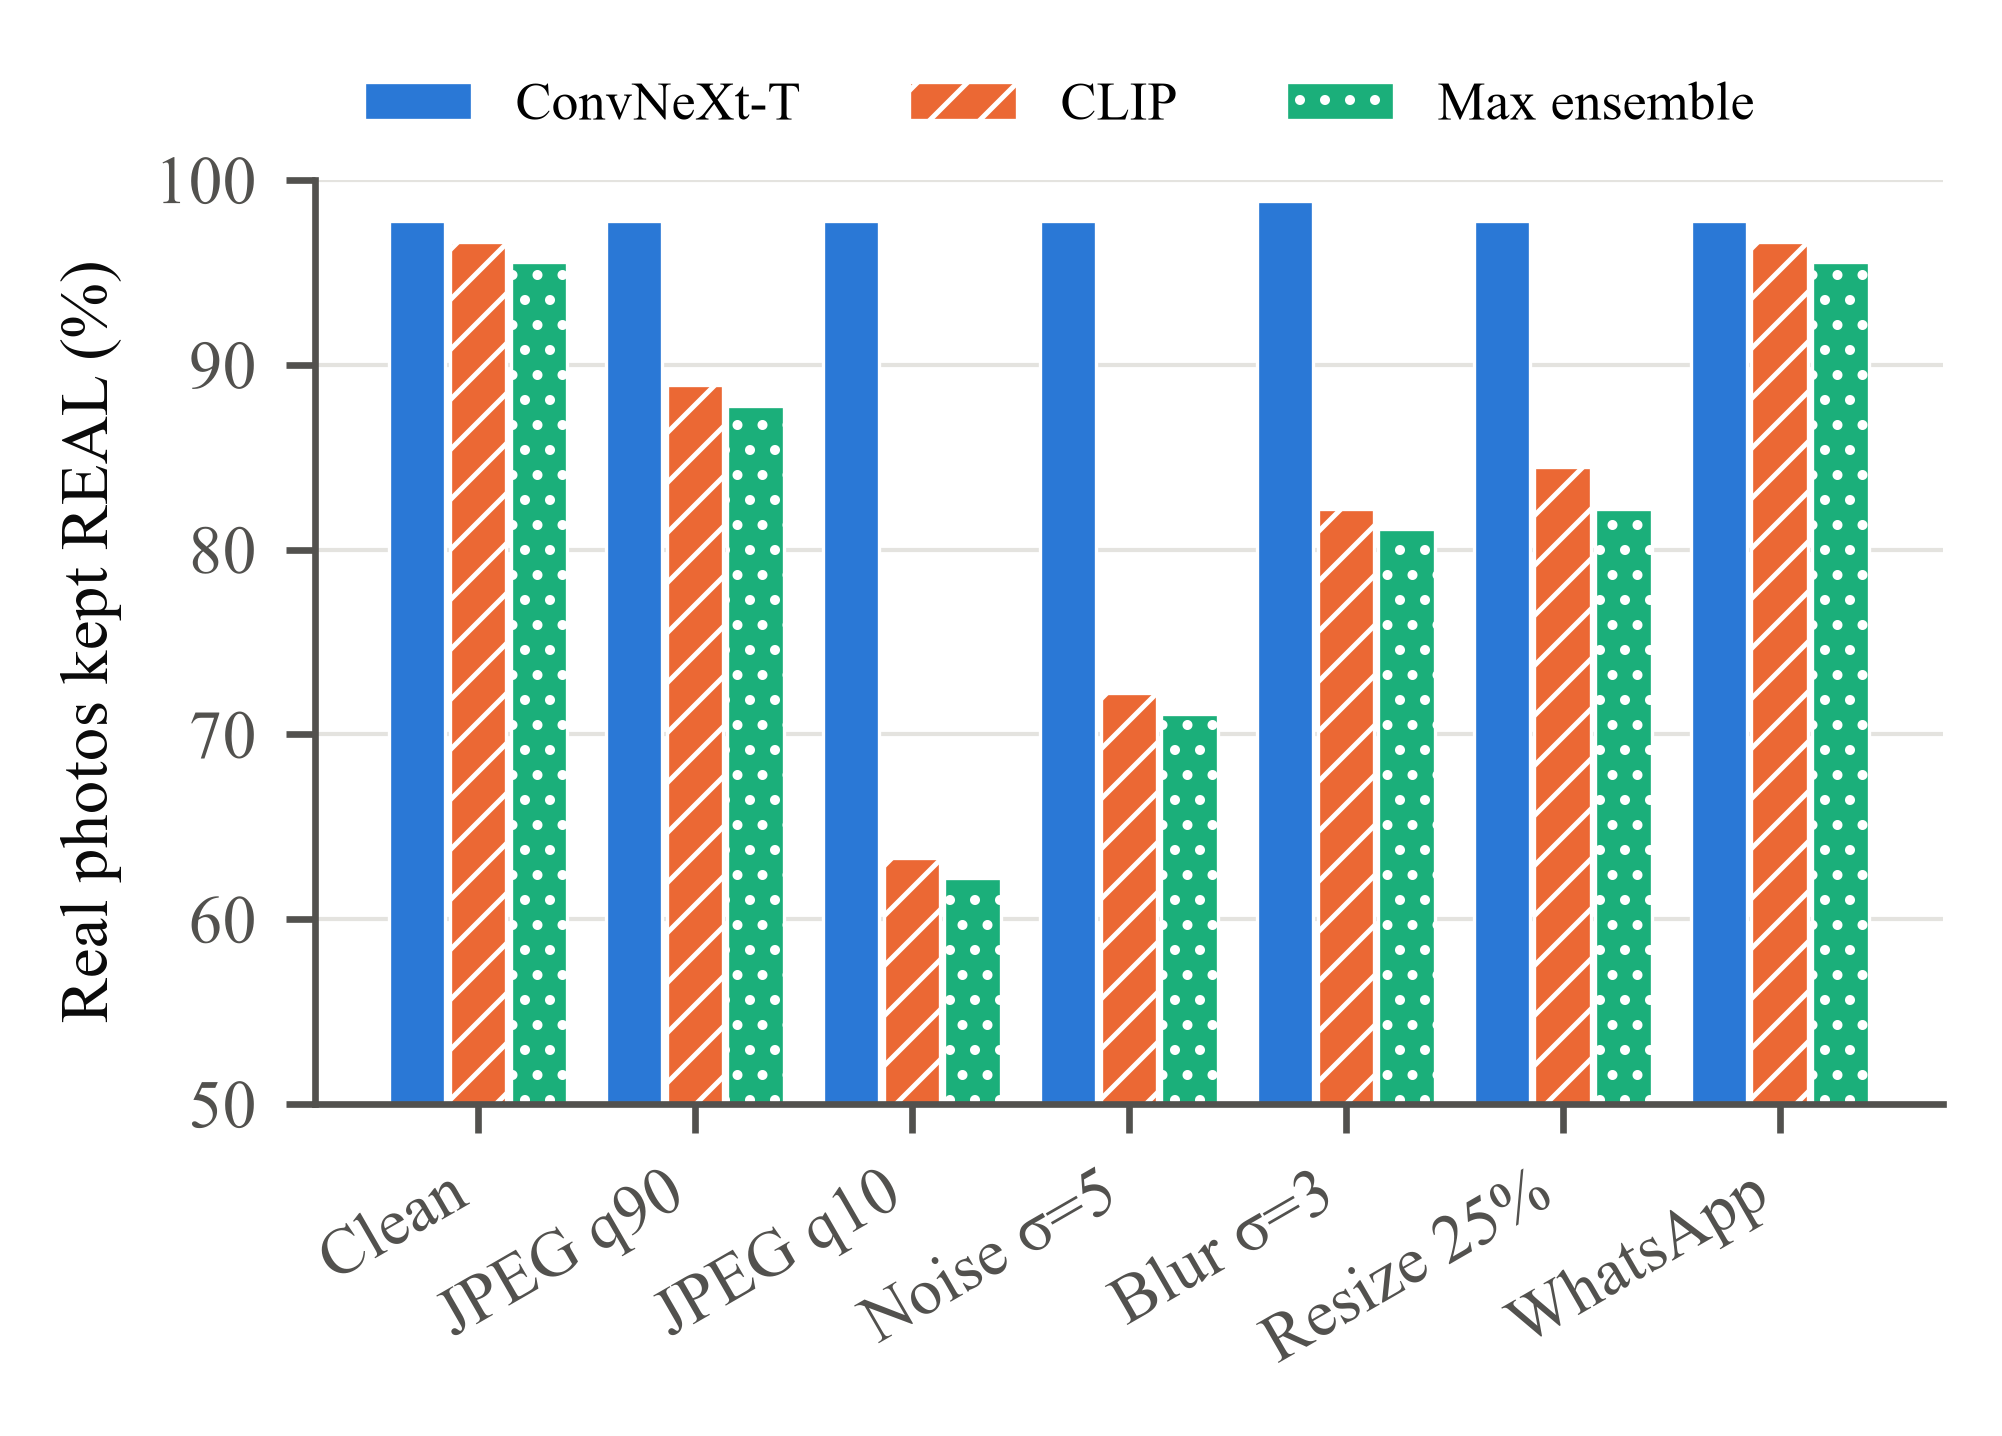
\includegraphics[width=\columnwidth]{figures/fig2_image_robustness.png}
\caption{Real-photo specificity of the image sub-models and the deployed max ensemble on 90 real images from seen sources under selected degradations.}
\label{fig-imgrob}
\end{figure}

Common sharing pipelines leave the image ensemble almost unaffected on seen sources: screenshot, WhatsApp-style and WebP processing all keep AUC at 0.99 or above. Fig. \ref{fig-imgrob} shows the exception: the CLIP sub-model raises false alarms on real photographs under faint noise and compression. The ensemble's real-photo specificity falls from 95.6\% (clean) to 87.8\% at JPEG quality 90, 71.1\% at noise std 5 and 62.2\% at quality 10. ConvNeXt alone stays between 96.7\% and 98.9\% in all 21 settings. The opposite happens under heavy blur (sigma 3): ConvNeXt catches only 50\% of fakes, and the ensemble recovers to 83.3\% because CLIP still detects them. The maximum rule therefore inherits CLIP's false alarms and ConvNeXt's misses, each under different degradations.

\begin{figure}[!t]
\centering
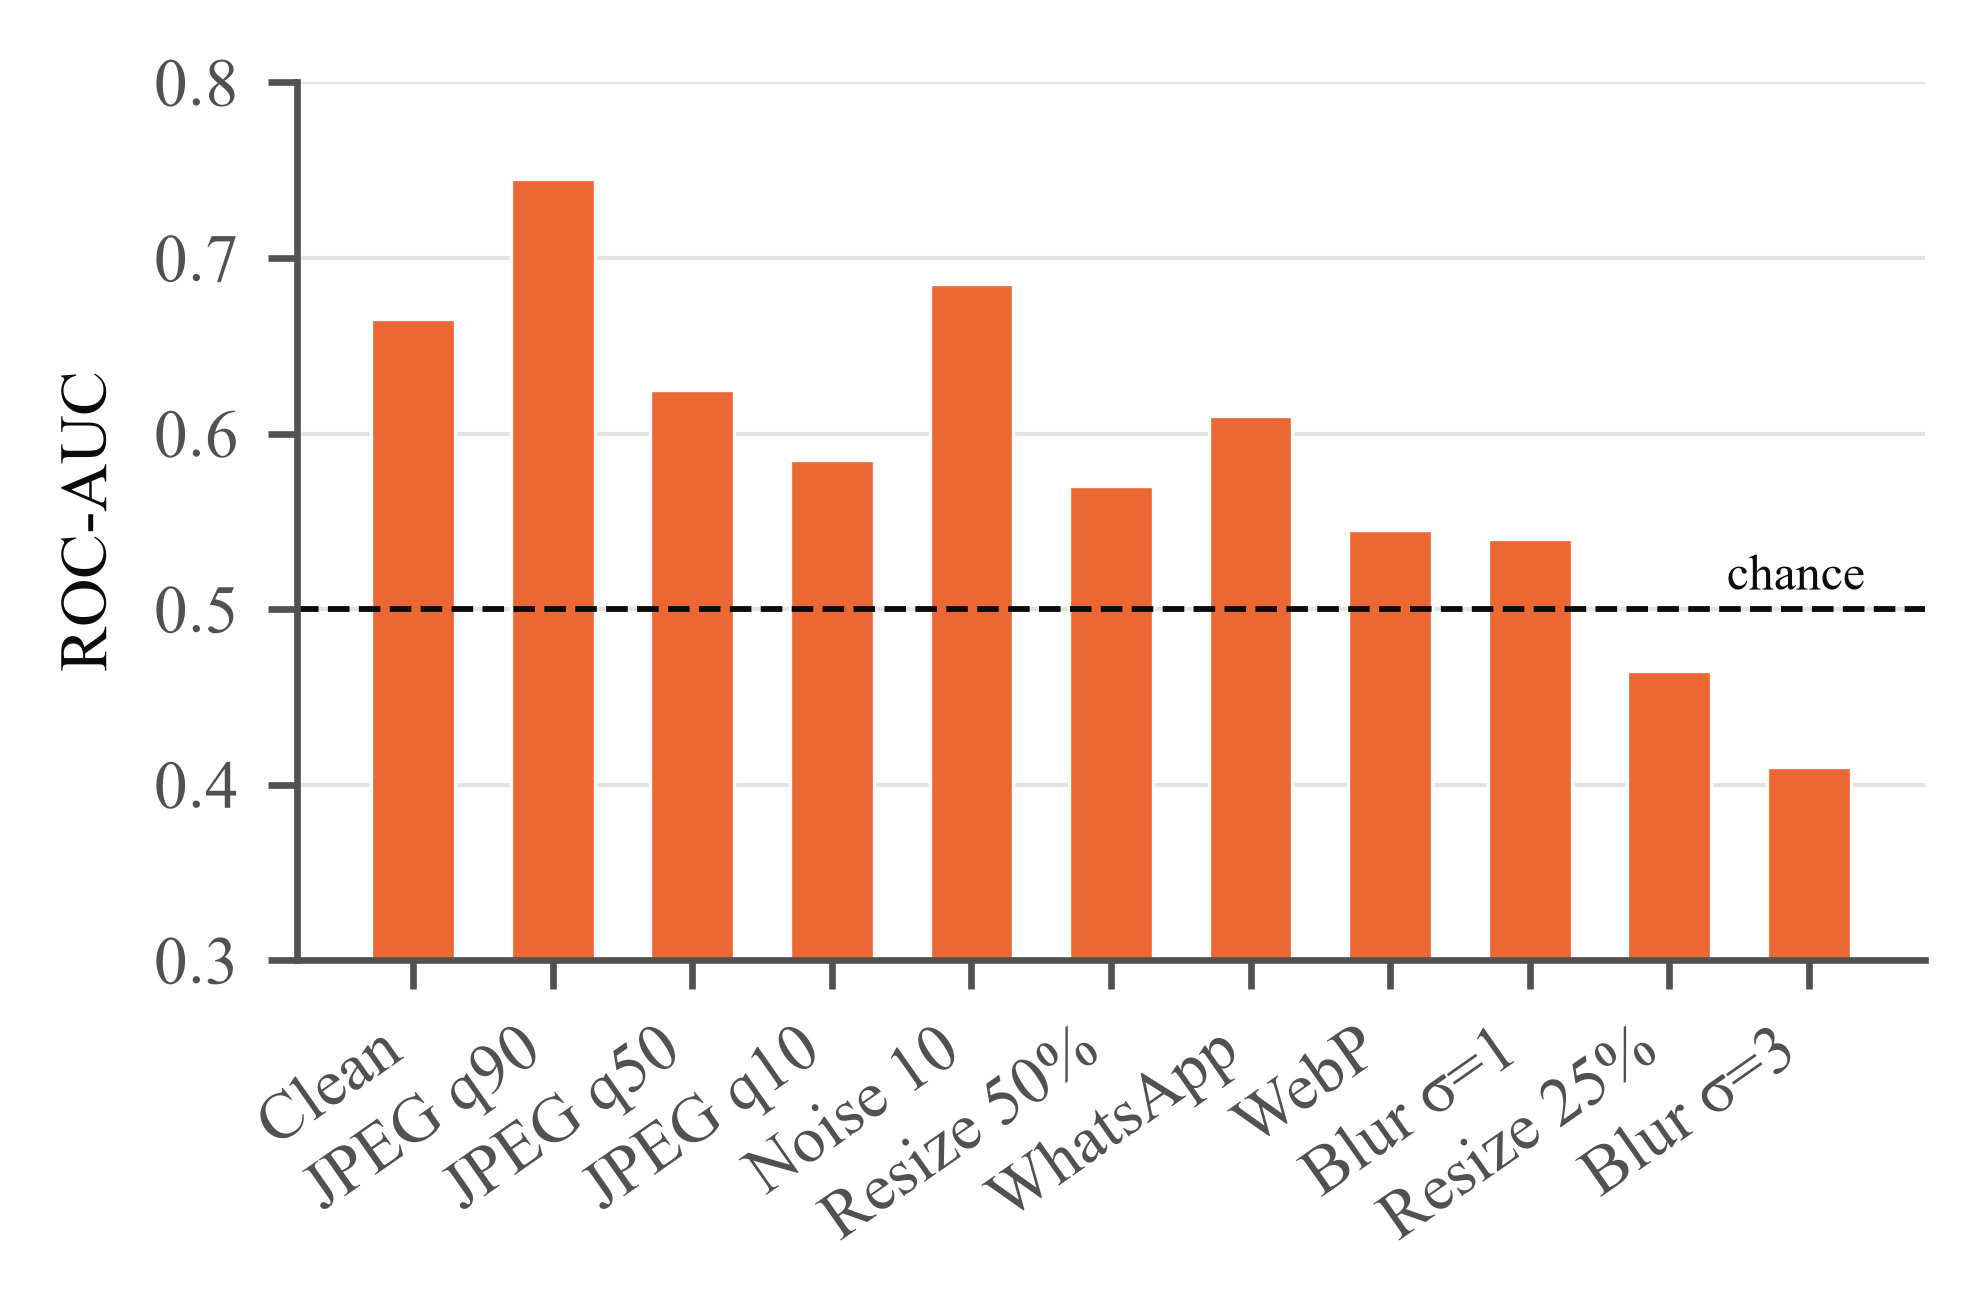
\includegraphics[width=\columnwidth]{figures/fig3_video_robustness.png}
\caption{Video model ROC-AUC on 30 RTFS clips with every sampled frame degraded. The dashed line marks chance.}
\label{fig-vidrob}
\end{figure}

Video is far more fragile (Fig. \ref{fig-vidrob}). At JPEG quality 10 the model labels every degraded fake REAL (fake recall 0\%). Blur with sigma 3 and 4$\times$ down-scaling push AUC below 0.5, which means the score now points the wrong way. WhatsApp-style processing alone drops AUC to 0.61. This 30-clip subset starts lower than the 300-clip headline (clean AUC 0.665), so the trend rather than the absolute value is the finding. Because shared video is nearly always re-compressed, clean benchmark numbers probably overstate how the model performs on the footage users actually see.

\subsection{Explanations, Provenance and Calibration}
\emph{Faithfulness.} For 195 fakes that ConvNeXt scores as FAKE, masking the 20\% of the image that Grad-CAM ranks highest reduced the FAKE probability by 0.232 on average, compared with 0.044 for a random mask of the same area. The Grad-CAM mask had the larger effect on 85\% of images, so the maps do point at regions the score depends on.

\emph{Provenance.} Across the 6,532 evaluation images, only 0.4\% of AI images carry any AI declaration, because benchmark datasets are re-encoded and stripped. The signal is valuable exactly where the detectors fail, however. All eight ChatGPT images carry OpenAI Content Credentials declaring AI generation. Their signatures are valid and the files are unchanged since signing, although the signer is not yet on the C2PA trust list. In total, 9 of the 1,026 AI images the ensemble misses declare themselves as AI-generated. The declaration survived a byte-for-byte copy in 8 of 8 cases and every re-encode we tried in 0 of 8 cases. ELA statistics separate real from fake with AUC 0.53--0.75 on most sources but 0.995 on DeepDetect. That points to a JPEG-history shortcut in this dataset that the classifiers may also be exploiting.

\begin{table}[!t]
\renewcommand{\arraystretch}{1.15}
\caption{Expected calibration error before and after temperature scaling.}
\label{tab-cal}
\centering
\footnotesize
\setlength{\tabcolsep}{3pt}
\begin{tabular}{>{\raggedright\arraybackslash}p{0.22\columnwidth}>{\raggedright\arraybackslash}p{0.17\columnwidth}>{\raggedright\arraybackslash}p{0.15\columnwidth}>{\raggedright\arraybackslash}p{0.18\columnwidth}>{\raggedright\arraybackslash}p{0.20\columnwidth}}
\hline
\textbf{Modality} & \textbf{n} & \textbf{T} & \textbf{ECE raw} & \textbf{ECE scaled} \\
\hline
Image & 6,500 & 4.45 & 0.158 & 0.056 \\
Video & 300 & 0.116 & 0.254 & 0.059 \\
\hline
\end{tabular}
\end{table}

\emph{Calibration.} Both detectors are mis-calibrated in their raw form (Table \ref{tab-cal}). The image model is over-confident ($T>1$): unseen fakes receive confident REAL scores. The video model's scores sit close to its threshold ($T<1$). Temperature scaling reduces ECE by about two-thirds in both cases. These post-scaling values were measured on the same scores used for fitting, so they are optimistic. A held-out calibration split is needed before they can be quoted as generalisation figures.

\subsection{Error Rates Across Demographic Groups}
To check whether genuine photos of some groups are wrongly flagged more often, we scored 600 real UTKFace~\cite{utkface} portraits, 60 per gender-race group. The deployed ensemble's specificity is 94.8\% overall but ranges from 90.0\% to 100\% across groups. ConvNeXt alone spans 96.7--100\% and CLIP alone 91.7--100\%. CLIP's two weakest groups are exactly the ensemble's two weakest, which again points to CLIP as the source of the false alarms. With 60 images per group the ranking of specific groups is noisy. The size of the spread and the sub-model it comes from are the reliable findings.


\section{Discussion and Limitations}
The results support one main lesson. A detector that scores 98\% on benchmark-like data can be close to chance on the next generator, and a user cannot tell which situation applies to their file. For that reason TruthLens describes REAL as ``no evidence of generation found'' rather than ``authentic'', reserves FAKE for clear scores, and places provenance and explanations beside the number. Several limitations remain.

\begin{itemize}
\item \emph{Training-data coverage.} Photorealistic GPT-class images and consumer face-swap apps are absent from every training source, and both are confirmed blind spots.
\item \emph{Dataset shortcuts.} DeepDetect's compression history, GenImage's JPEG-versus-PNG format split and RTFS's different encodes for real and fake clips may all inflate the measured accuracy.
\item \emph{Small samples.} The blind-spot sets (8 and 15 images), our own videos (10), the video robustness subset (30) and the per-group fairness samples (60) support qualitative conclusions only.
\item \emph{Robustness.} No detector has been retrained with the compression augmentation that Section VI-D calls for, and audio robustness is untested.
\item \emph{Engineering.} Job state lives in one server process, so horizontal scaling needs a shared queue, and inference is CPU-only in our deployment.
\end{itemize}

A forensic tool can cause harm in two directions. A false FAKE can be used to discredit a genuine photograph, and a false REAL can lend credibility to a hoax. The verdict bands, explicit conflict notes, ``lead, not proof'' wording and the absence of any automated action on a verdict are our mitigations. The tool should not be used for legal, employment or safety decisions without human review.


\section{Conclusion and Future Work}
TruthLens shows that a modest team can build a working multimodal detection service that provides evidence alongside its scores, and that measuring such a system honestly is as much work as building it. Its detectors are near-perfect on familiar data and unreliable on unfamiliar generators, and the video model degrades badly under ordinary compression. Provenance metadata fills some of the gaps when it survives. Our next steps follow directly from these measurements: retrain with more diverse generators (GPT-class images, Flux and consumer face-swap apps) and with compression and noise augmentation; evaluate audio under the same degradations; fit calibration on a held-out split; extend the per-group analysis to video and audio; and study audio-visual fusion such as lip-sync consistency for talking-head forgeries.

\section*{Acknowledgment}
The authors thank Prof. Dhanashree Tamhane and the Department of Information Technology, Vidyalankar Institute of Technology, Mumbai, for guidance and support throughout this project.

\begin{thebibliography}{00}
\bibitem{ffpp} A. R\"ossler, D. Cozzolino, L. Verdoliva, C. Riess, J. Thies, and M. Nie{\ss}ner, ``FaceForensics++: Learning to detect manipulated facial images,'' in \emph{Proc. IEEE/CVF Int. Conf. Comput. Vis. (ICCV)}, 2019, pp. 1--11.
\bibitem{celebdf} Y. Li, X. Yang, P. Sun, H. Qi, and S. Lyu, ``Celeb-DF: A large-scale challenging dataset for DeepFake forensics,'' in \emph{Proc. IEEE/CVF Conf. Comput. Vis. Pattern Recognit. (CVPR)}, 2020, pp. 3207--3216.
\bibitem{cifake} J. J. Bird and A. Lotfi, ``CIFAKE: Image classification and explainable identification of AI-generated synthetic images,'' \emph{IEEE Access}, vol. 12, pp. 15642--15650, 2024.
\bibitem{genimage} M. Zhu \emph{et al.}, ``GenImage: A million-scale benchmark for detecting AI-generated image,'' in \emph{Adv. Neural Inf. Process. Syst. (NeurIPS), Datasets and Benchmarks Track}, 2023.
\bibitem{asvspoof2019} X. Wang \emph{et al.}, ``ASVspoof 2019: A large-scale public database of synthesized, converted and replayed speech,'' \emph{Comput. Speech Lang.}, vol. 64, Art. no. 101114, 2020.
\bibitem{wang2020} S.-Y. Wang, O. Wang, R. Zhang, A. Owens, and A. A. Efros, ``CNN-generated images are surprisingly easy to spot... for now,'' in \emph{Proc. IEEE/CVF Conf. Comput. Vis. Pattern Recognit. (CVPR)}, 2020, pp. 8695--8704.
\bibitem{ojha2023} U. Ojha, Y. Li, and Y. J. Lee, ``Towards universal fake image detectors that generalize across generative models,'' in \emph{Proc. IEEE/CVF Conf. Comput. Vis. Pattern Recognit. (CVPR)}, 2023, pp. 24480--24489.
\bibitem{frank2020} J. Frank, T. Eisenhofer, L. Sch\"onherr, A. Fischer, D. Kolossa, and T. Holz, ``Leveraging frequency analysis for deep fake image recognition,'' in \emph{Proc. Int. Conf. Mach. Learn. (ICML)}, 2020, pp. 3247--3258.
\bibitem{clip} A. Radford \emph{et al.}, ``Learning transferable visual models from natural language supervision,'' in \emph{Proc. Int. Conf. Mach. Learn. (ICML)}, 2021, pp. 8748--8763.
\bibitem{convnext} Z. Liu, H. Mao, C.-Y. Wu, C. Feichtenhofer, T. Darrell, and S. Xie, ``A ConvNet for the 2020s,'' in \emph{Proc. IEEE/CVF Conf. Comput. Vis. Pattern Recognit. (CVPR)}, 2022, pp. 11976--11986.
\bibitem{dfdc} B. Dolhansky \emph{et al.}, ``The DeepFake Detection Challenge (DFDC) dataset,'' \emph{arXiv preprint} arXiv:2006.07397, 2020.
\bibitem{wilddeepfake} B. Zi, M. Chang, J. Chen, X. Ma, and Y.-G. Jiang, ``WildDeepfake: A challenging real-world dataset for deepfake detection,'' in \emph{Proc. 28th ACM Int. Conf. Multimedia}, 2020, pp. 2382--2390.
\bibitem{efficientnet} M. Tan and Q. V. Le, ``EfficientNet: Rethinking model scaling for convolutional neural networks,'' in \emph{Proc. Int. Conf. Mach. Learn. (ICML)}, 2019, pp. 6105--6114.
\bibitem{aasist} J.-w. Jung \emph{et al.}, ``AASIST: Audio anti-spoofing using integrated spectro-temporal graph attention networks,'' in \emph{Proc. IEEE Int. Conf. Acoust., Speech Signal Process. (ICASSP)}, 2022, pp. 6367--6371.
\bibitem{inthewild} N. M. M\"uller, P. Czempin, F. Dieckmann, A. Froghyar, and K. B\"ottinger, ``Does audio deepfake detection generalize?'' in \emph{Proc. Interspeech}, 2022, pp. 2783--2787.
\bibitem{wav2vec2} A. Baevski, Y. Zhou, A. Mohamed, and M. Auli, ``wav2vec 2.0: A framework for self-supervised learning of speech representations,'' in \emph{Adv. Neural Inf. Process. Syst. (NeurIPS)}, vol. 33, 2020, pp. 12449--12460.
\bibitem{tak2022} H. Tak, M. Todisco, X. Wang, J.-w. Jung, J. Yamagishi, and N. Evans, ``Automatic speaker verification spoofing and deepfake detection using wav2vec 2.0 and data augmentation,'' in \emph{Proc. Odyssey: The Speaker and Language Recognition Workshop}, 2022, pp. 112--119.
\bibitem{gradcam} R. R. Selvaraju, M. Cogswell, A. Das, R. Vedantam, D. Parikh, and D. Batra, ``Grad-CAM: Visual explanations from deep networks via gradient-based localization,'' in \emph{Proc. IEEE Int. Conf. Comput. Vis. (ICCV)}, 2017, pp. 618--626.
\bibitem{simonyan2014} K. Simonyan, A. Vedaldi, and A. Zisserman, ``Deep inside convolutional networks: Visualising image classification models and saliency maps,'' in \emph{Proc. Int. Conf. Learn. Represent. (ICLR) Workshop}, 2014.
\bibitem{c2pa} Coalition for Content Provenance and Authenticity, ``C2PA technical specification,'' version 2.1, 2024. [Online]. Available: https://c2pa.org/specifications/
\bibitem{ldm} R. Rombach, A. Blattmann, D. Lorenz, P. Esser, and B. Ommer, ``High-resolution image synthesis with latent diffusion models,'' in \emph{Proc. IEEE/CVF Conf. Comput. Vis. Pattern Recognit. (CVPR)}, 2022, pp. 10684--10695.
\bibitem{invisiblewm} ShieldMnt, ``invisible-watermark: Python library for invisible image watermarking,'' GitHub repository. [Online]. Available: https://github.com/ShieldMnt/invisible-watermark
\bibitem{krawetz2007} N. Krawetz, ``A picture's worth: Digital image analysis and forensics,'' presented at \emph{Black Hat Briefings USA}, 2007.
\bibitem{guo2017} C. Guo, G. Pleiss, Y. Sun, and K. Q. Weinberger, ``On calibration of modern neural networks,'' in \emph{Proc. Int. Conf. Mach. Learn. (ICML)}, 2017, pp. 1321--1330.
\bibitem{aivshuman} alessandrasala79, ``AI vs. human-generated images,'' Kaggle dataset, 2025. [Online]. Available: https://www.kaggle.com/datasets/alessandrasala79/ai-vs-human-generated-dataset
\bibitem{faces140k} xhlulu, ``140k real and fake faces,'' Kaggle dataset, 2020. [Online]. Available: https://www.kaggle.com/datasets/xhlulu/140k-real-and-fake-faces
\bibitem{deepdetect} ayushmandatta1, ``DeepDetect-2025,'' Kaggle dataset, 2025. [Online]. Available: https://www.kaggle.com/datasets/ayushmandatta1/deepdetect-2025
\bibitem{diffusiondb} Z. J. Wang, E. Montoya, D. Munechika, H. Yang, B. Hoover, and D. H. Chau, ``DiffusionDB: A large-scale prompt gallery dataset for text-to-image generative models,'' in \emph{Proc. 61st Annu. Meeting Assoc. Comput. Linguistics (ACL)}, 2023, pp. 893--911.
\bibitem{violajones} P. Viola and M. Jones, ``Rapid object detection using a boosted cascade of simple features,'' in \emph{Proc. IEEE Comput. Soc. Conf. Comput. Vis. Pattern Recognit. (CVPR)}, 2001, pp. I-511--I-518.
\bibitem{deepvoice} J. J. Bird and A. Lotfi, ``Real-time detection of AI-generated speech for DeepFake voice conversion,'' \emph{arXiv preprint} arXiv:2308.12734, 2023.
\bibitem{librispeech} V. Panayotov, G. Chen, D. Povey, and S. Khudanpur, ``Librispeech: An ASR corpus based on public domain audio books,'' in \emph{Proc. IEEE Int. Conf. Acoust., Speech Signal Process. (ICASSP)}, 2015, pp. 5206--5210.
\bibitem{vcc2020} Y. Zhao \emph{et al.}, ``Voice Conversion Challenge 2020: Intra-lingual semi-parallel and cross-lingual voice conversion,'' in \emph{Proc. Joint Workshop Blizzard Challenge and Voice Conversion Challenge}, 2020, pp. 80--98.
\bibitem{openfake} sanketghadge1, ``OpenFake data (20k images),'' Kaggle dataset, 2025. [Online]. Available: https://www.kaggle.com/datasets/sanketghadge1/openfake-data-20k-img
\bibitem{rtfs} ``RealTimeFaceSwap-10k (RTFS-10k),'' Hugging Face dataset, 2025. [Online]. Available: https://huggingface.co/datasets/stplusplus/rtfs-10k
\bibitem{utkface} Z. Zhang, Y. Song, and H. Qi, ``Age progression/regression by conditional adversarial autoencoder,'' in \emph{Proc. IEEE Conf. Comput. Vis. Pattern Recognit. (CVPR)}, 2017, pp. 5810--5818.
\bibitem{hendrycks2019} D. Hendrycks and T. Dietterich, ``Benchmarking neural network robustness to common corruptions and perturbations,'' in \emph{Proc. Int. Conf. Learn. Represent. (ICLR)}, 2019.
\end{thebibliography}

\end{document}
